\section{Tutorial}
\label{section:tutorial}

Here is a tutorial walk-through of some small projects with
\sft{ssu-align}. To follow along with this tutorial, move into the
\prog{ssu-align-0.1/} subdirectory of \prog{infernal-1.01/} directory
where you unpacked and built the \sft{infernal} package. Once there
create a new directory, something like \prog{my-tutorial} and move
into it. The instructions in this tutorial assume that you have the
\prog{ssu-align-0.1/ssu-align} perl script and
\sft{easel} programs in \prog{infernal-1.01/easel/miniapps/} in your
\$PATH. For example, you should be able to run \prog{ssu-align},
\prog{esl-alimanip} and \prog{esl-reformat} by simply typing
\prog{ssu-align}, \prog{esl-alimanip} or \prog{esl-alimanip} at the
UNIX prompt.  These instructions also assume that you have setup your
local \prog{ssu-align-0.1/sa-0p1.params} file to include your local
paths. Instructions on how to do all of this are included in the
Installation section.

\begin{comment}
The instructions in this tutorial assume that you
have the \sft{ssu-align} perl script and \sft{easel} programs in your
path. For example, you should be able to run \emph{version 1.01} of
\prog{ssu-align} and \prog{esl-alimanip} by simply typing
\prog{ssu-align} or \prog{esl-alimanip} at the UNIX prompt.  The
instructions also assume that you have setup your local
\prog{sa-0p1.params} to include your local paths to the executables.
Instructions on how to do all of this are included in the the
Installation section. Frequently, I will refer to files included in
the distrubution. To specify their locations, I will use the strings
\prog{\$INFDIR} and \prog{\$SADIR} to refer to the top-level
\prog{infernal-1.01} directory and its \prog{ssu-align-0.1}
subdirectly respectively.
\end{comment}
%One final note: for many of the small
%tutorials below I ask you to copy files into new directories before
%performing the tutorials, this is not good practice, you could just 

\subsection{Files used in this tutorial}

In the first section of this tutorial we'll use the following files:

  \begin{sreitems}{}
  \item[\prog{ssu-align-0.1/seeds/ssu3-0p1.cm}] A covariance model (CM) file that
    defines three SSU rRNA CMs: an archael model, a bacterial model,
    and a eukaryotic model. These are the three default models used by
    \sft{ssu-align}. More information can be found on these models
    in section~\ref{section:chap9}.
  \item[\prog{ssu-align-0.1/tutorial/seed-15.fa}] a sequence file containing
    fifteen SSU rRNA sequences, created specifically for use in this tutorial.
  \item[\prog{ssu-align-0.1/sa-0p1.params}] A file containing paths to
    \sft{infernal} executable files that \sft{ssu-align} needs
    to run. You will likely need to change
    these paths to point to where you've installed the \prog{cmsearch}
    and \prog{cmalign} programs as noted in the Installation section.
  \end{sreitems}

Other files will be explained as needed in the later sections of the tutorial.
%Create a new directory that you can work in, and copy the three
%files listed above there. I'll assume for the following examples that you've
%installed the \prog{ssu-align} PERL script in your path; if not, you'll
%need to give a complete path name to the script (e.g. something like
%\newline
%\prog{/usr/people/nawrocki/infernal-1.01/ssu-align-0.1/ssu-align} 
%instead of just \prog{ssu-align}).

\subsection{Creating structural SSU alignments with \sft{ssu-align}}

First, we'll go through how to use the program for
it's most basic and fundamental purpose, creating multiple
alignments of SSU rRNA sequences. 

The file \prog{seed-15.fa} contains five archaeal sequences, five
bacterial sequences and five eukaryotic sequences from the
\sft{ssu-align} v0.1 seed alignments. These seed alignments
were derived from alignments from the \db{CRW} database
\cite{CannoneGutell02} as described in section~\ref{section:chap9}.
This sequence file was created to allow a quick demonstration of
\sft{ssu-align}'s ability to create structurally annotated multiple
alignments of SSU sequences. To run this example, 
execute the following command:

\scriptuser{ssu-align ../seeds/ssu3-0p1.cm ../tutorial/seed-15.fa seed-15 ../sa-0p1.params}\\

As you can see, the \sft{ssu-align} script takes four command line
arguments. The first is a CM file. The default CM file
\prog{ssu3-0p1.cm} contains three CMs: an archaeal SSU model, a
bacterial SSU model and a eukaryotic SSU model. The second argument is
the target sequence file to search (this must be in FASTA format). The
third is a string that is used as the basis for naming output
files. In this case, the script will create a new directory called
\prog{seed-15} where all output files will be created; \prog{seed-15}
will also be included as a prefix to the names of all output files.

\newpage

The program will first print a header describing the program version
used, command used, current date, and some other information. 
The following information printed to the screen:

\begin{sreoutput}
# ssu-align :: define and align SSU rRNA sequences
# SSU-ALIGN 0.1 (June 2009)
# Copyright (C) 2009 HHMI Janelia Farm Research Campus
# Freely distributed under the GNU General Public License (GPLv3)
# - - - - - - - - - - - - - - - - - - - - - - - - - - - - - - - - - - - -
# command: wd-1p0-branch/ssu-align-0.1/ssu-align -F ssu3-0p1.cm seed-15.fa seed-15 sa-0p1.params
# date:    Thu Aug 20 06:32:04 2009
#
# Stage 1: Determining SSU start/end positions and best matching models.
\end{sreoutput}

In stage 1, the program scans the input sequences with each of the
three models in the CM file \\ \prog{ssu3-0p1.cm}. This has two
purposes.  First, it classifies each sequence by determining which
model in the input CM file is its ``best-matching'' model, defined as
the model that gives the sequence the highest primary sequence-based
alignment score using a profile HMM. Secondly, it
defines the start and end points of the SSU sequences based on the
best-matching model's alignment.

Stage 1 takes about 20 seconds on this dataset (on an Intel Xeon 3.0
GHz processor, which I'll use for all example runs in this
guide). When it finishes you'll see: 

\begin{sreoutput}
# Stage 1: Determining SSU start/end positions and best matching models.
#
# output file name            description                                
# --------------------------  -------------------------------------------
  seed-15.tab                 locations/scores of hits defined by HMM(s)
  seed-15.archaea.hits.list   list of sequences to align with archaea CM
  seed-15.archaea.hits.fa           5 sequences to align with archaea CM
  seed-15.bacteria.hits.list  list of sequences to align with bacteria CM
  seed-15.bacteria.hits.fa          5 sequences to align with bacteria CM
  seed-15.eukarya.hits.list   list of sequences to align with eukarya CM
  seed-15.eukarya.hits.fa           5 sequences to align with eukarya CM
\end{sreoutput}

This lists and briefly describes the seven new files the script created
in a newly created subdirectory of the current working dir called
\prog{seed-15/}. The content and format of these files are described
in detail in section~\ref{section:output}. For now a brief explanation
should be sufficient. The first file \prog{seed-15.tab} is output from
\sft{infernal}'s \prog{cmsearch} program. The other six files are
model-specific: two files for each model that was the best-matching
model for at least one sequence in the input target sequence file
\prog{seed-15.fa}. The \prog{.hits.list} suffixed files contain a list
of the sequences that match best to the model, and the \prog{.hits.fa}
suffixed files are those actual sequences. If any of the models had
not been the best-matching model to at least one target sequence,
there would be no \prog{.hits.list} or \prog{.hits.fa} files for that
model.

The program will now proceed to stage 2, the alignment stage. This
stage serially progresses through each model that was the
best-matching model for at least one sequence and uses the model to
align the best-matching sequences. The alignments are computed by scoring
a combination of both sequence and secondary structure conservation,
as opposed to the scoring in stage one which only used sequence
conservation. As the alignment to each model finishes, two new lines
of text, one for each of two newly created files, will appear on the
screen. For this example, alignment to all three models takes about 20
seconds. When it finishes you'll see:

\newpage

\begin{sreoutput}
#
# Stage 2: Aligning each sequence to it's best matching model.
#
# output file name            description
# --------------------------  -------------------------------------------
  seed-15.archaea.stk         archaea alignment
  seed-15.archaea.cmalign     archaea cmalign output
  seed-15.bacteria.stk        bacteria alignment
  seed-15.bacteria.cmalign    bacteria cmalign output
  seed-15.eukarya.stk         eukarya alignment
  seed-15.eukarya.cmalign     eukarya cmalign output
  seed-15.scores              list of CM/HMM scores for each sequence
  seed-15.log                 log file (*this* text printed to stdout)
#
# All output files created in directory ./seed-15/
#
# CPU time (search):     00:00:15
# CPU time (alignment):  00:00:21
# CPU time (total):      00:00:37
#
\end{sreoutput}

The newly created alignments are the \prog{.stk} suffixed files. These
were created by \sft{infernal}'s \prog{cmalign} program. The
\prog{cmalign} output is in the \prog{.cmalign} suffixed files.  As in
stage 1, these files were created in the \prog{./seed-15/}
subdirectory. 

\subsubsection{Description of alignments}

Section~\ref{section:output} contains more information
on \sft{ssu-align} output files, but for now we'll focus only on the new
alignments.  Take a look at the archaeal alignment we just created in
\prog{seed-15/seed-15.archaea.stk}.

This alignment includes consensus secondary structure annotation and
is in \emph{Stockholm format}. 
Stockholm format, the native alignment format used by \sft{hmmer} and
\sft{infernal} and the \db{pfam} and \db{rfam}
databases, is documented in detail in the \sft{infernal} user's
guide which is included as a PDF in \prog{infernal-1.01/}

For now, what you need to know about the key features of the alignment file is:
\begin{itemize}

\item The alignment is in an interleaved format, like other
  common alignment file formats such as \sft{clustalw}.
  Lines consist of a name, followed by an aligned sequence;
  the alignment is split into blocks separated by blank lines.

\item Gaps are indicated by the characters ., \_, -, or \verb+~+.
  Many SSU alignments will have large regions of 100\% gaps at the
  beginning and ends of the alignment. 
  This will happen if the sequences are 
  partial SSU sequences, such as those  obtained with PCR
  primers that target well conserved regions within the SSU
  molecule.

\item Special lines starting with {\small\verb+#=GR+} followed by a
  sequence name and then {\small\verb+POST+} contain posterior
  probabilities for each aligned residue for the sequence they
  correspond to. These are confidence estimates in the correctness of
  the alignment.  The POSTX. row indicates the ’tens’ place of the
  confidence estimate while POST.X row indicates the ’ones’ place. So
  the confidence estimate for a residue with 9 in the POSTX. row, and
  7 in the POST.X row to two significant digits is 97\%. This means that
  if you sampled alignments from the posterior distribution of all
  possible alignments of this sequence to the model, about 97% of the
  time that residue would appear in that of the alignment. One special
  case: if the posterior probability is very nearly 100% (it’s
  difficult to be more precise on the exact percentage due to
  numerical precision issues) the annotated posterior values will be
  ``*'' characters in both the tens and ones places. These confidence
  estimates can be used to mask the alignment to remove columns with
  significant fractions of ambiguously aligned residues as demonstrated
  below.

\item A special line starting with {\small\verb+#=GC SS_cons+}
  indicates the secondary structure consensus. Gap characters annotate
  unpaired (single-stranded) columns. Base pairs are indicated by any
  of the following pairs: \verb+<>+, \verb+()+, \verb+[]+, or
  \verb+[]+.

\item A special ``RF'' line starting with {\small\verb+#=GC RF+}
  indicates the consensus, or ReFerence, model. Gaps in the RF line
  are \emph{insert} columns, where at least 1 sequence has at least 1
  inserted residue between two consensus positions. Uppercase residues
  in the RF line are well conserved positions in the model; lowercase
  residues are less well conserved.
\end{itemize}

\subsubsection{converting Stockholm alignments to FASTA format}

Two steps are required to convert a Stockholm alignment to an aligned
FASTA formatted file that includes gap characters. First you must
convert a \prog{ssu-align} output alignment to a special
non-interleaved Stockholm formatted file using the
\prog{esl-reformat} program. To convert our archaeal alignment:

\user{esl-reformat -o new.stk pfam seed-15/seed-15.archaea.stk}

The second step is to use the \sft{perl} script \prog{stk2fa.pl}
provided in the \prog{scripts/} subdirectory of \prog{ssu-align-0.1/}
to create a FASTA file. To see the usage of this script, do:

\user{perl scripts/stk2fa.pl}
\begin{sreoutput}
usage: perl stk2fa.pl [-options] <non-interleaved stockholm alnment (1 line per seq)>

Options:
	-C : include #=GC <x> markup, named as "GC-<x>"
	-R : include #=GR <x> <tag> markup, named as "GR-<x>-tag"

Note that the stockholm alignment must be non-interleaved.
You can convert an interleaved ssu-align/cmalign output alignment "foo.stk"
to non-interleaved "foo2.stk" with "esl-reformat -o foo2.stk pfam foo.stk"
\end{sreoutput}

To convert our \prog{new.stk} alignment to the FASTA file
\prog{new.fa}, do:

\user{perl scripts/stk2fa.pl new.stk > new.fa}

Note that this will remove the \prog{\#=GC} markup, which includes the
consensus secondary structure (\prog{\#=GC SS\_cons}) and reference
(consensus) sequence (\prog{\#=GC RF}) as well as the posterior
probability annotation. To include those, as listed above in the
script's usage, use the \prog{-C} and/or \prog{-R} options to the
script.

\subsection{Creating masks for pruning alignments with the
  \prog{esl-alimanip} program}

If your goal is to use a phylogenetic inference program to build trees
from alignments created by \sft{ssu-align}, you may want to mask
out columns of the alignment that may include misaligned residues
first, and then only run the inference on the remaining columns where
you're confident the alignment is correct. 

As mentioned above, \sft{infernal}'s \prog{cmalign} program
can automatically calculate posterior probabilities that estimate the
level of ambiguity in the alignment of each residue. These can be
interpreted as how confident the model is in each aligned residue in
each sequence and are useful for finding and
removing ambiguously aligned regions prior to phylogenetic inference.
The \prog{esl-alimanip} program can be used to mask
\sft{ssu-align} generated alignments based on these confidence estimates.

I recommend a three step masking process. The first step is to remove
all insert columns from the alignment. Insert columns include residues
that are literally \emph{not aligned}, but rather just inserted in
between the appropriate two consensus positions. 
%(There's more explanation of this in the ``Background'' section).  
Since inserts are
not aligned they should not be included in a phylogenetic inference.
The second step is to create a mask of the consensus model based on
the confidence estimates in the alignment. The final step is to prune
the alignment based on that mask.

Here's an example of using \prog{esl-alimanip} for the three steps. 
First, we'll use \prog{esl-alimanip} to remove all insert columns and
save the new alignment to \prog{seed-15.archaea.noins.stk}:

\user{esl-alimanip -k -o seed-15.archaea.noins.stk seed-15/seed-15.archaea.stk}

%(Note: if \prog{esl-alimanip} is not in your path, you'll have to
%specify the full path to the program. For example:
%\prog{/usr/people/nawrocki/infernal-1.01/easel/miniapps/esl-alimanip}.

The program will create the new alignment file
\prog{seed-15.archaea.noins.stk} almost instantly. 
The \prog{-k} option to \prog{esl-alimanip} tells it to remove all
columns of the alignment that are gaps in the \prog{\#\=GC RF}
annotation. In \sft{ssu-align} generated alignments, gaps in the
\prog{\#\=GC RF} annotation indicate a column is an insert column that
does not correspond to a consensus model position.

Next, we'll generate a mask based on the alignment confidence estimates
in the insert-removed alignment :

\user{esl-alimanip --omask my.mask --p-rf --pfract 0.95 --pthresh
  0.95 \\   -o trash.stk seed-15.archaea.noins.stk}

(Note that the full command includes both lines above. Many of the
commands in the rest of this tutorial are too long for a single line,
and are split up like this one.)
The following will print to the screen:

\begin{sreoutput}
Average posterior value:                            0.98877 (6219 non-gap residues)
Average posterior value in non-gap #=GC RF columns: 0.98877 (6219 non-gap RF residues)

1449 of 1508 RF columns (0.961) pass threshold
\end{sreoutput}

And the mask file \prog{my.mask} is created. Take a look at this
file. It is a single line of text of length $1508$ characters,
containing only \prog{0}s and \prog{1}s. The length is 1508 because
the consensus archaeal model (see section~\ref{section:chap9}) is 1508 residues
long. A \prog{0} at position \prog{n} indicates that consensus position \prog{n}
will excluded (pruned away) when the mask is applied. A \prog{1} at
position \prog{n} indicates that consensus position \prog{n} will be included (not
pruned away) when the mask is applied. In this mask file there are
$1449$ \prog{1}s and $59$ \prog{0s}.

In general the columns where the alignment confidence is high will be
included, and where it is low will be excluded. More specifically, a
column \prog{n} is included if at least 0.95 fraction (95\%)
of the sequences that have a residue (non-gap) in column \prog{n} have a
confidence estimate of 0.95 or better for that residue. All other
columns are excluded.

Using 0.95 for both \prog{--p-fract} and \prog{--p-thresh} are the
recommended options for masking. Section~\ref{section:chap9} 
describes a simple experiment testing how different thresholds affect
alignment accuracy, and using 0.95 for both thresholds resulted in 
high accuracy (see Table~\ref{tbl:kolbe09-pp}).
However, these thresholds can be changed using command-line options to 
\prog{esl-alimanip}. The fraction threshold can be changed to
\prog{<x>} with the \prog{--pfract <x>} and the confidence estimate
threshold can be changed to \prog{<y>} with the \prog{--pthresh <y>}
option.

Note that only non-gap residues are considered when the mask is
generated. This means if a consensus column only has a single residue
in it, and it has high confidence (say 0.98), then that column will be
be included in the mask (not be pruned away). This may be be
undesirable, depending on what type of downstream phylogenetic inference
you are going to do. Many phylogenetic inference programs treat gaps
as missing data, and for such programs you may want to exclude very gappy
columns when masking. 

The \prog{esl-alimanip} program can also take the gappiness of a
column into account when masking. To use the same confidence estimate
thresholds as the previous \prog{esl-alimanip} mask generation
(\prog{--pfract 0.95 --pthresh 0.95}) but \emph{also} exclude any column 
with more than 45\% gaps, execute the command:

\user{esl-alimanip --omask my2.mask -g --gapthresh 0.45 --p-rf
  --pfract 0.95 \\ --pthresh 0.95 -o trash.stk seed-15.archaea.noins.stk}

\begin{sreoutput}
Average posterior value:                            0.98877 (6219 non-gap residues)
Average posterior value in non-gap #=GC RF columns: 0.98901 (6184 non-gap RF residues)

1435 of 1467 RF columns (0.978) pass threshold
\end{sreoutput}

The final line indicates that $1467$ consensus positions had less
than 45\% gaps, of these $1435$ passed the confidence estimate
thresholds. The new mask \prog{my2.mask} is still $1508$ characters
long, but now contains only $1435$ \prog{1}s.

The final step of masking is applying the mask. This is also done with
\prog{esl-alimanip}:

\user{esl-alimanip -k --mask-rf my2.mask -o
  my2.masked.archaea.stk \\ seed-15.archaea.noins.stk}

The new alignment is saved in \prog{my2.masked.archaea.stk}.

The easel program \prog{esl-alistat} can be used to calculate and
display some summary statistics of the new alignment:

\user{esl-alistat my2.masked.archaea.stk}

\begin{sreoutput}
Alignment number:    1
Format:              Stockholm
Number of sequences: 5
Alignment length:    1435
Total # residues:    6069
Smallest:            857
Largest:             1435
Average length:      1213.8
Average identity:    82%
\end{sreoutput}

The \prog{ssu-align-0.1/scripts/} directory includes three simple
\sft{perl} scripts that may be useful for getting information on mask
files created with \prog{esl-alimanip}. The \prog{summarize\_mask.pl}
script reports on the number of {0}s and {1}s in a mask. The
\prog{rename\_mask.pl} script will copy a mask to a file with a name
that includes the number of {1}s and length of a mask. The
\prog{compare\_equiwidth\_masks.pl} script will compare and report on
the overlap of two masks that have the same number of total characters
(same number of {0}s plus {1}s). To get usage information on these
scripts, simply execute them with no arguments, for example:

\user{perl summarize\_mask.pl}


\subsection{Visualizing alignment masks}

The \prog{esl-ssudraw} program can be used to create a secondary
structure diagram that shows which parts of the SSU consensus model
are included and excluded by the mask. This requires the use of a
postscript template file for the archaeal model. This is provided in 
\\ \prog{ssu-align-0.1/seeds/ss-diagrams/archaea-0p1.ps}. 
%Copy that file into the working directory. To generate a diagram of our
%mask: 
To generate a diagram of our mask:

\user{esl-ssudraw --mask my2.mask --mask-col
  seed-15/seed-15.archaea.stk \\ ../seeds/ss-diagrams/archaea-0p1.ps my2.mask.ps}

The \prog{--mask} option tells \prog{esl-ssudraw} that we are
supplying the mask \prog{my2.mask} for display. The \prog{--mask-col}
option specifies the color scheme for the mask (other types of mask
coloring are demonstrated later in this tutorial. Additionally, 
\prog{esl-ssudraw} takes three command-line arguments. The first is
the alignment file that the mask pertains to. Note that we use
\prog{seed-15.archaea.stk}, this is the original alignment we created,
not the masked alignment. The second argument is the template
postscript file. Here we use \prog{archaea-0p1.ps} because it corresponds
to the \sft{ssu-align} 0.1 archaea CM, which we used to create this
alignment. The third argument is the desired name of the output
postscript file. The \prog{my2.mask.ps} file is created here, which
includes a drawing of the secondary structure diagram. You can either
display this using a postscript viewer, or convert it to a PDF using a
conversion program (I use the \prog{ps2pdf} program that is freely
available for download for most unices). Note that Mac OS/X's
automatic conversion with the \prog{Preview} program is not reliable
for converting these postscript files to PDFs.

The masked secondary structure diagram is displayed on the next page.
The color legend and other information on the diagram is meant to be
self explanatory. \prog{esl-ssudraw} can be used to draw secondary
structures displaying different types of information than masks, as
described next.

\newpage

\begin{figure}
\begin{center}
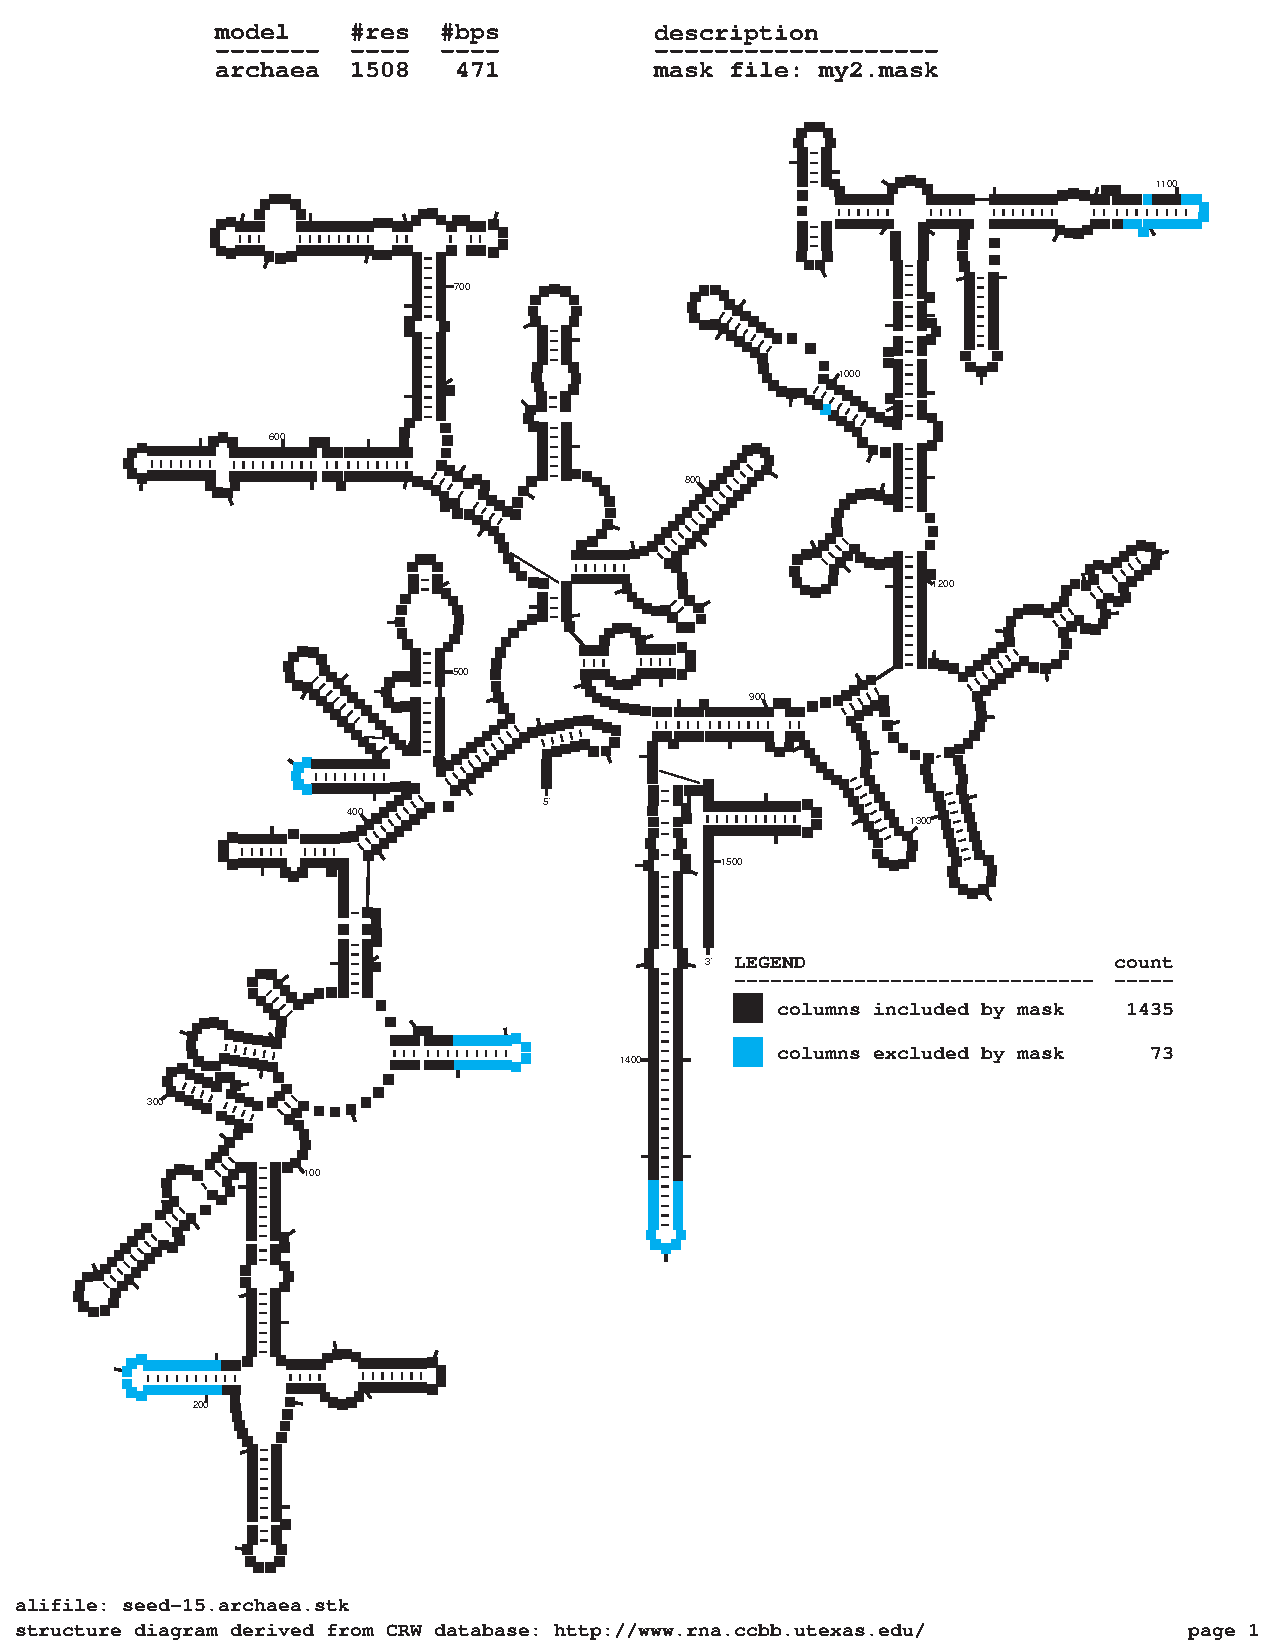
\includegraphics[width=5.7in]{Figures/my2-mask}
\end{center}
\caption{\textbf{The my2.mask.ps diagram that shows the my2.mask on
    the SSU archaeal consensus structure.}}
\end{figure}

\subsection{Visualizing alignments with \sft{esl-ssudraw}}

SSU rRNA alignments are large and difficult to view in a meaningful
way. The \prog{esl-ssudraw} program introduced for visualizing masks
earlier in this tutorial can be also used to display statistics of
a particular alignment on the consensus SSU secondary structure of the
model used to create the alignment. As before,
using \prog{esl-ssudraw} requires a template postscript file of the
consensus secondary structure. The template files for the 3 default
\textsc{ssu-align} version 0.1 seed models are included as
\prog{\$INFDIR/ssu-align-0.1/seeds/ss-diagrams/{archaea,bacteria,eukarya}-0p1.ps}. 
(Unfortunately, it is difficult to create new template files for
additional models you might build for your own analyses.) 

\prog{esl-ssudraw} can be run in two different modes. In the default
mode, \emph{alignment} mode, the structure diagrams will display
statistics on the alignment. In \emph{individual} mode, the structure
diagrams will show individual sequences in the alignment by displaying
the actual residues at each consensus position of the alignment. Note
that the diagrams are always of the consensus model defined in the
template file. In alignment mode, only statistics of consensus
positions are displayed. In individual mode, only residues that align to
consensus positions are displayed.

The following table summarizes the different statistics that can be
created in alignment mode.
An example of each of these types of
diagrams is included as the indicated figure for the default
eukaryotic seed alignment. The postscript and pdf files for each of
these included figures, as well as analogous diagrams for the
archaeal and bacterial seeds are included in 
\prog{\$INFDIR/ssu-align-0.1/seeds/ss-diagrams/}, named as indicated 
in the ``file'' column of the table. 

\begin{center}
\begin{tabular}{llll} \hline
\prog{esl-ssudraw} option(s) & statistic                     &  figure & file \\ \hline
\prog{<none>}                & information content           & \ref{fig:eukinfo} & \prog{eukarya-0p1-info} \\
& & & \\
\prog{--prog}                & average posterior probability & \ref{fig:eukprob} & \prog{eukarya-0p1-prob} \\
& & & \\
\prog{--ins}                 & frequency of insertions       & \ref{fig:eukins}   & \prog{eukarya-0p1-ins} \\
                             & after each position           & & \\
& & & \\
\prog{--dall}                & frequency of deletions        & \ref{fig:eukdall}  & \prog{eukarya-0p1-dall} \\
& & & \\
\prog{--dint}                & frequency of internal deletions & \ref{fig:eukdint}  & \prog{eukarya-0p1-dint} \\
                             & (excluding terminal deletions)  & & \\
& & & \\
\prog{--struct}              & additional information from     & \ref{fig:eukstruct} & \prog{eukarya-0p1-struct} \\
                             & conserved structure \\
\end{tabular}
\end{center}

As an example of how these files were created, the command

\user{esl-ssudraw --dall eukarya-0p1.stk eukarya-0p1.ps eukarya-0p1-dall.ps}

was used to create Figure~\ref{fig:eukdall} (after copying the seed alignment
in \prog{\$INFDIR/ssu-align-0.1/seeds/eukarya-0p1.stk} and the template file 
\prog{\$INFDIR/ssu-align-0.1/seeds/ss-diagrams/eukarya-0p1.ps} to the current 
working directory.)

\newpage

\begin{figure}
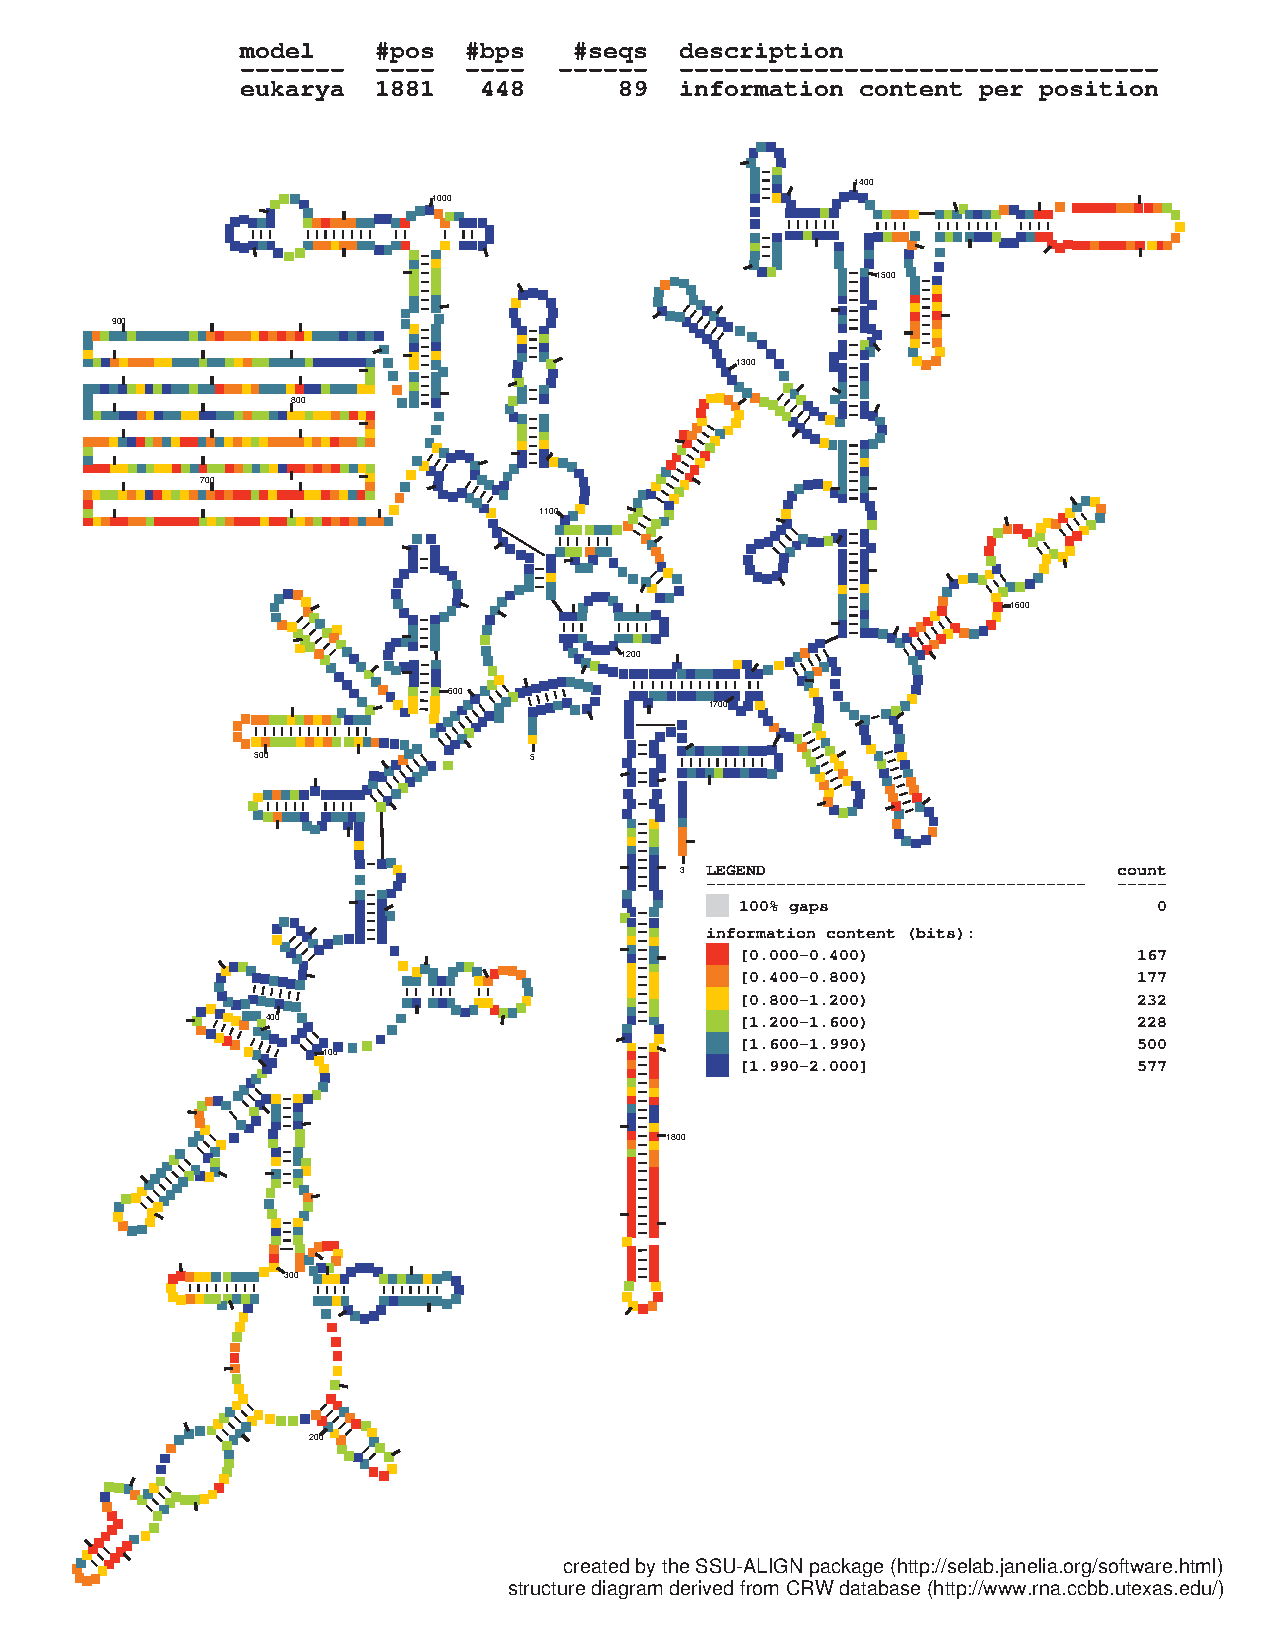
\includegraphics[height=8.5in]{Figures/eukarya-0p1-info}
\label{fig:eukinfo}
\end{figure}

\newpage

\begin{figure}
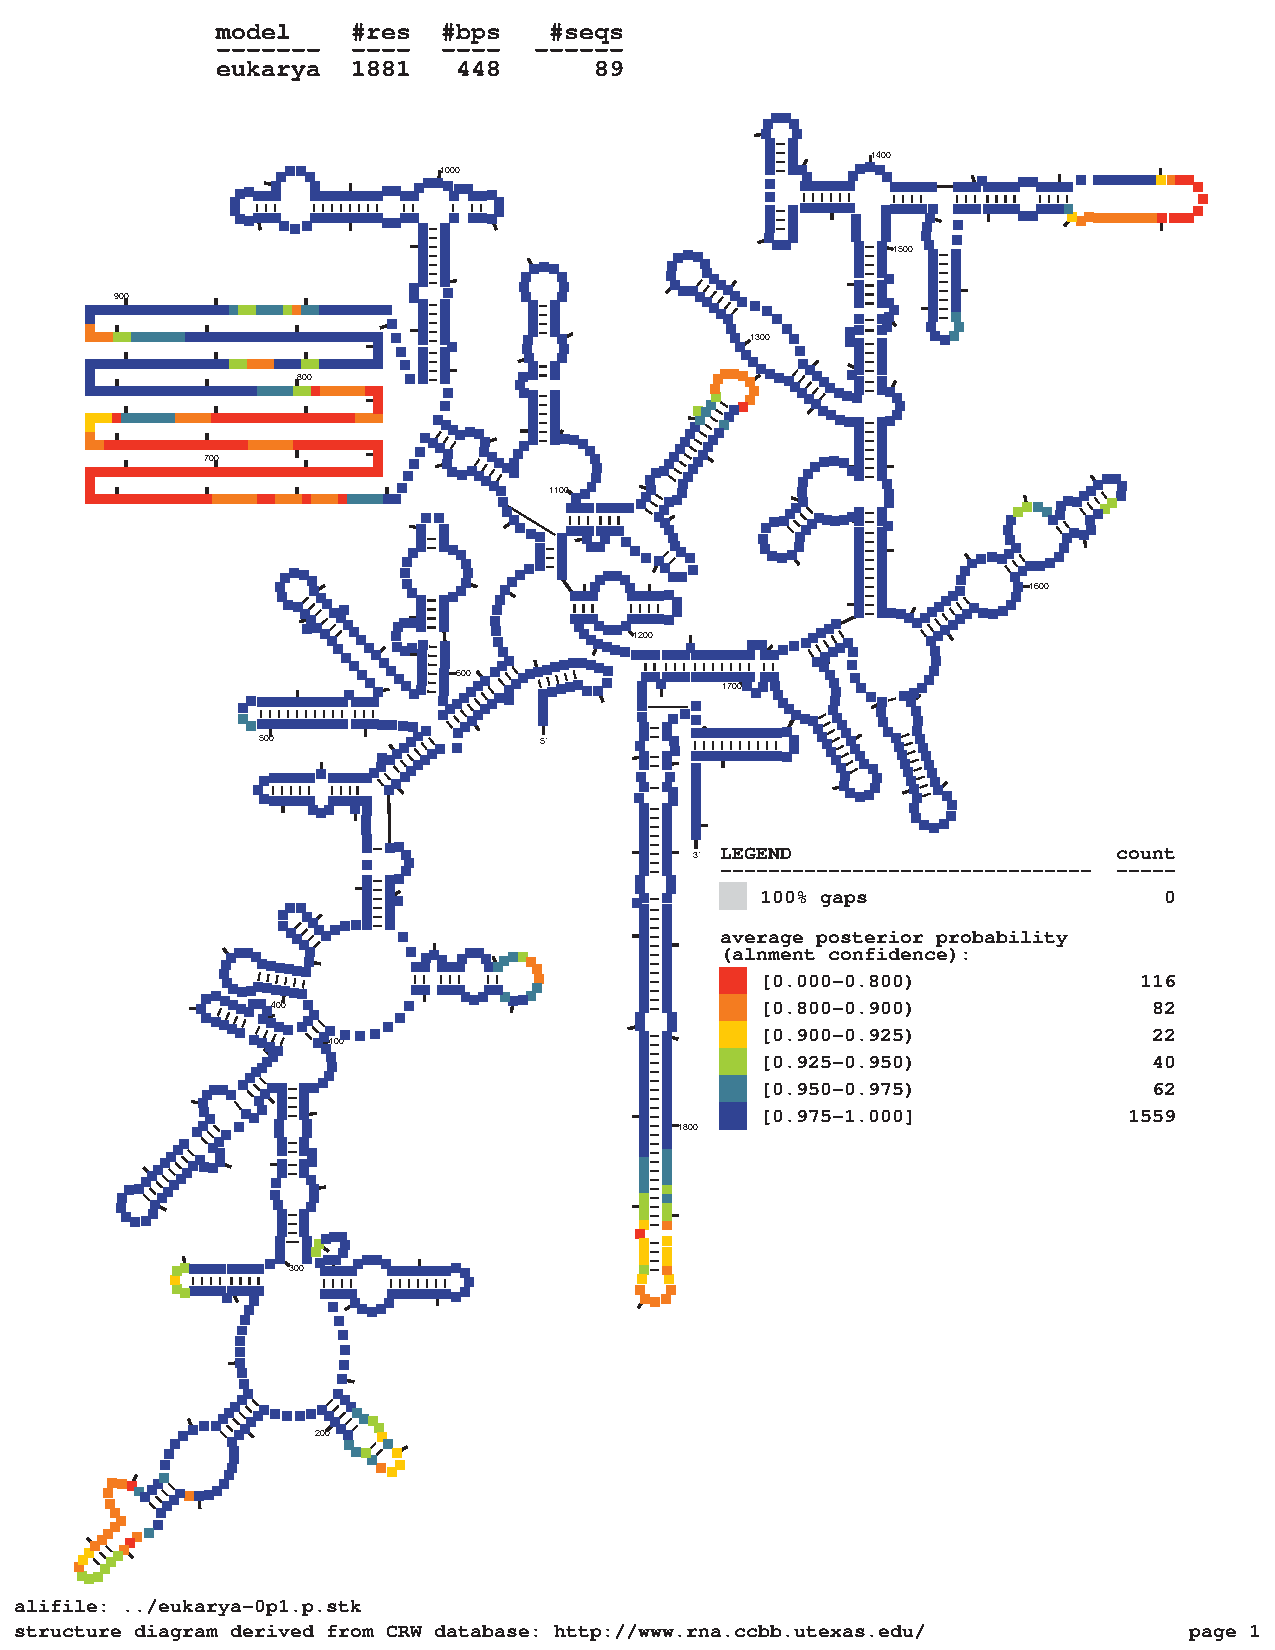
\includegraphics[height=8.5in]{Figures/eukarya-0p1-prob}
\label{fig:eukinfo}
\end{figure}

\newpage

\begin{figure}

\includegraphics[height=8.5in]{Figures/eukarya-0p1-ins}
\label{fig:eukinfo}
\end{figure}

\newpage

\begin{figure}
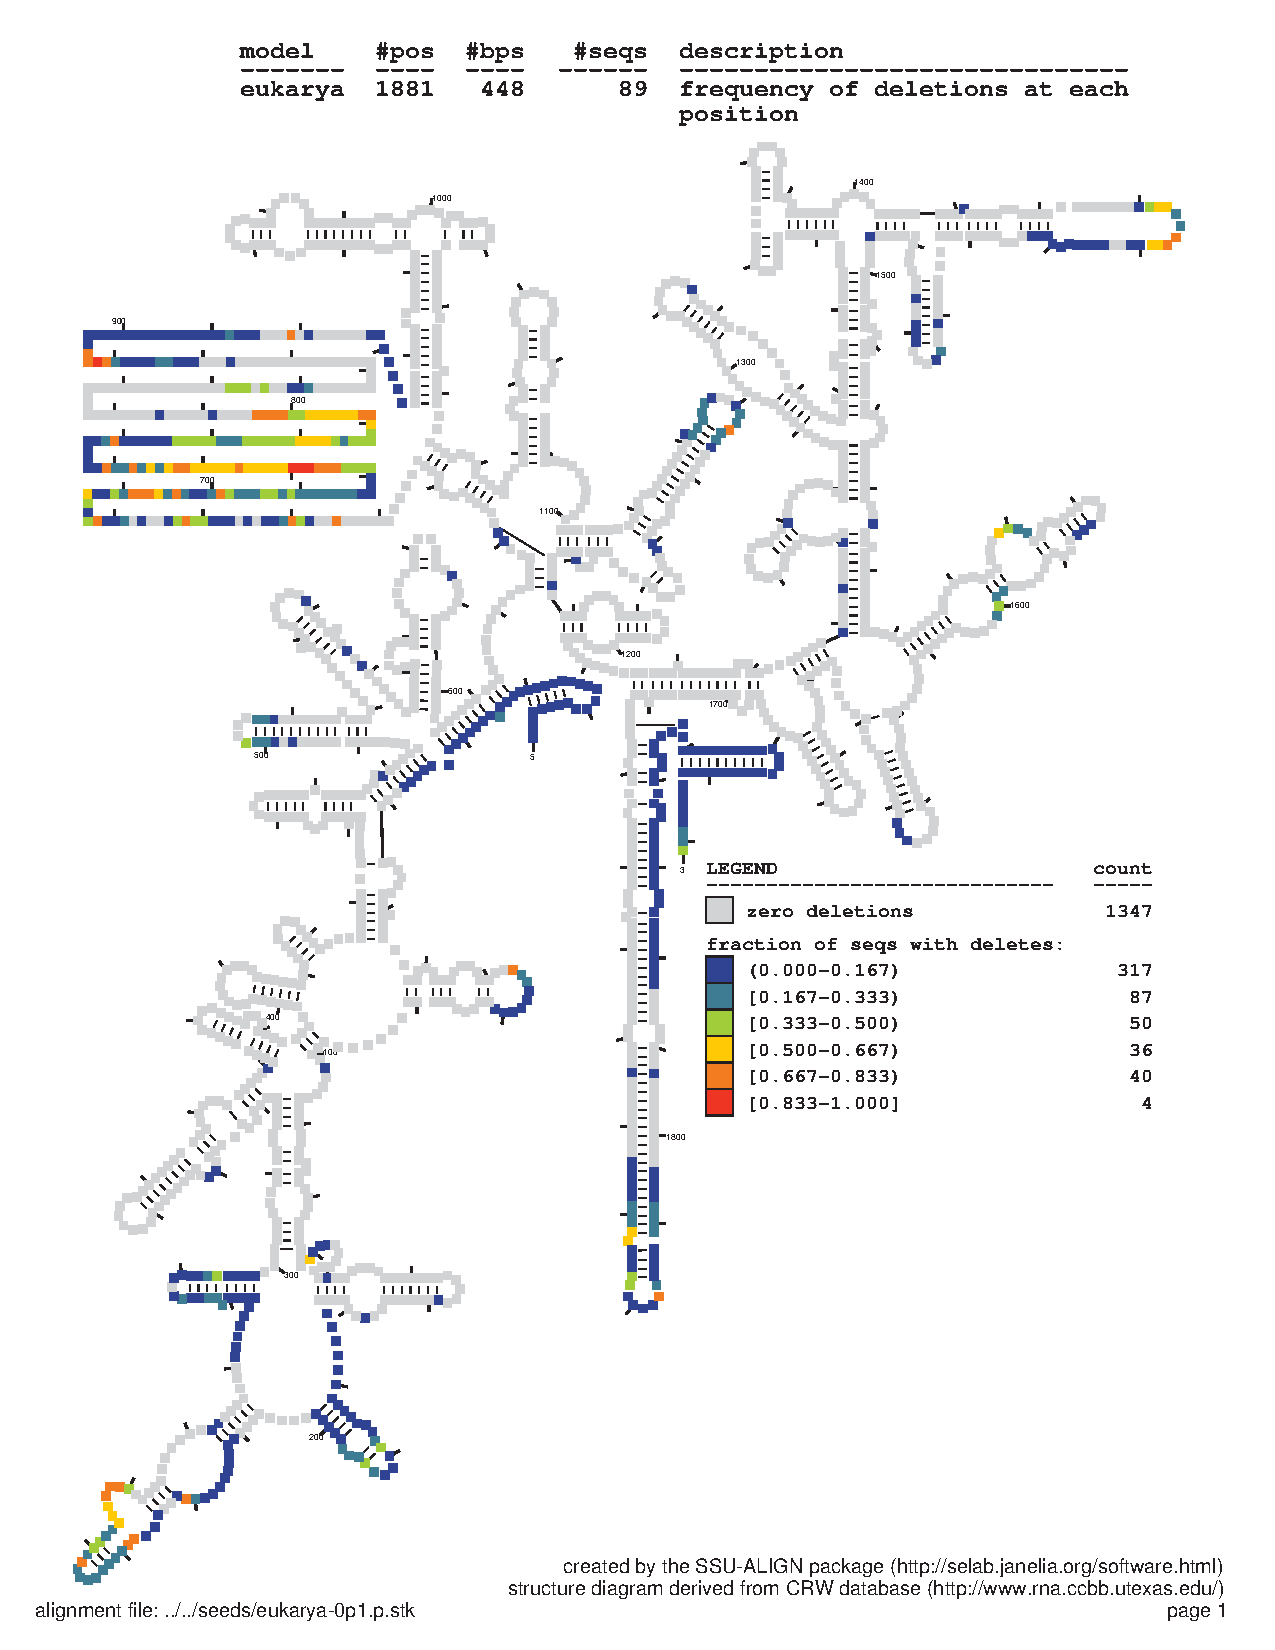
\includegraphics[height=8.5in]{Figures/eukarya-0p1-dall}
\label{fig:eukinfo}
\end{figure}

\newpage

\begin{figure}
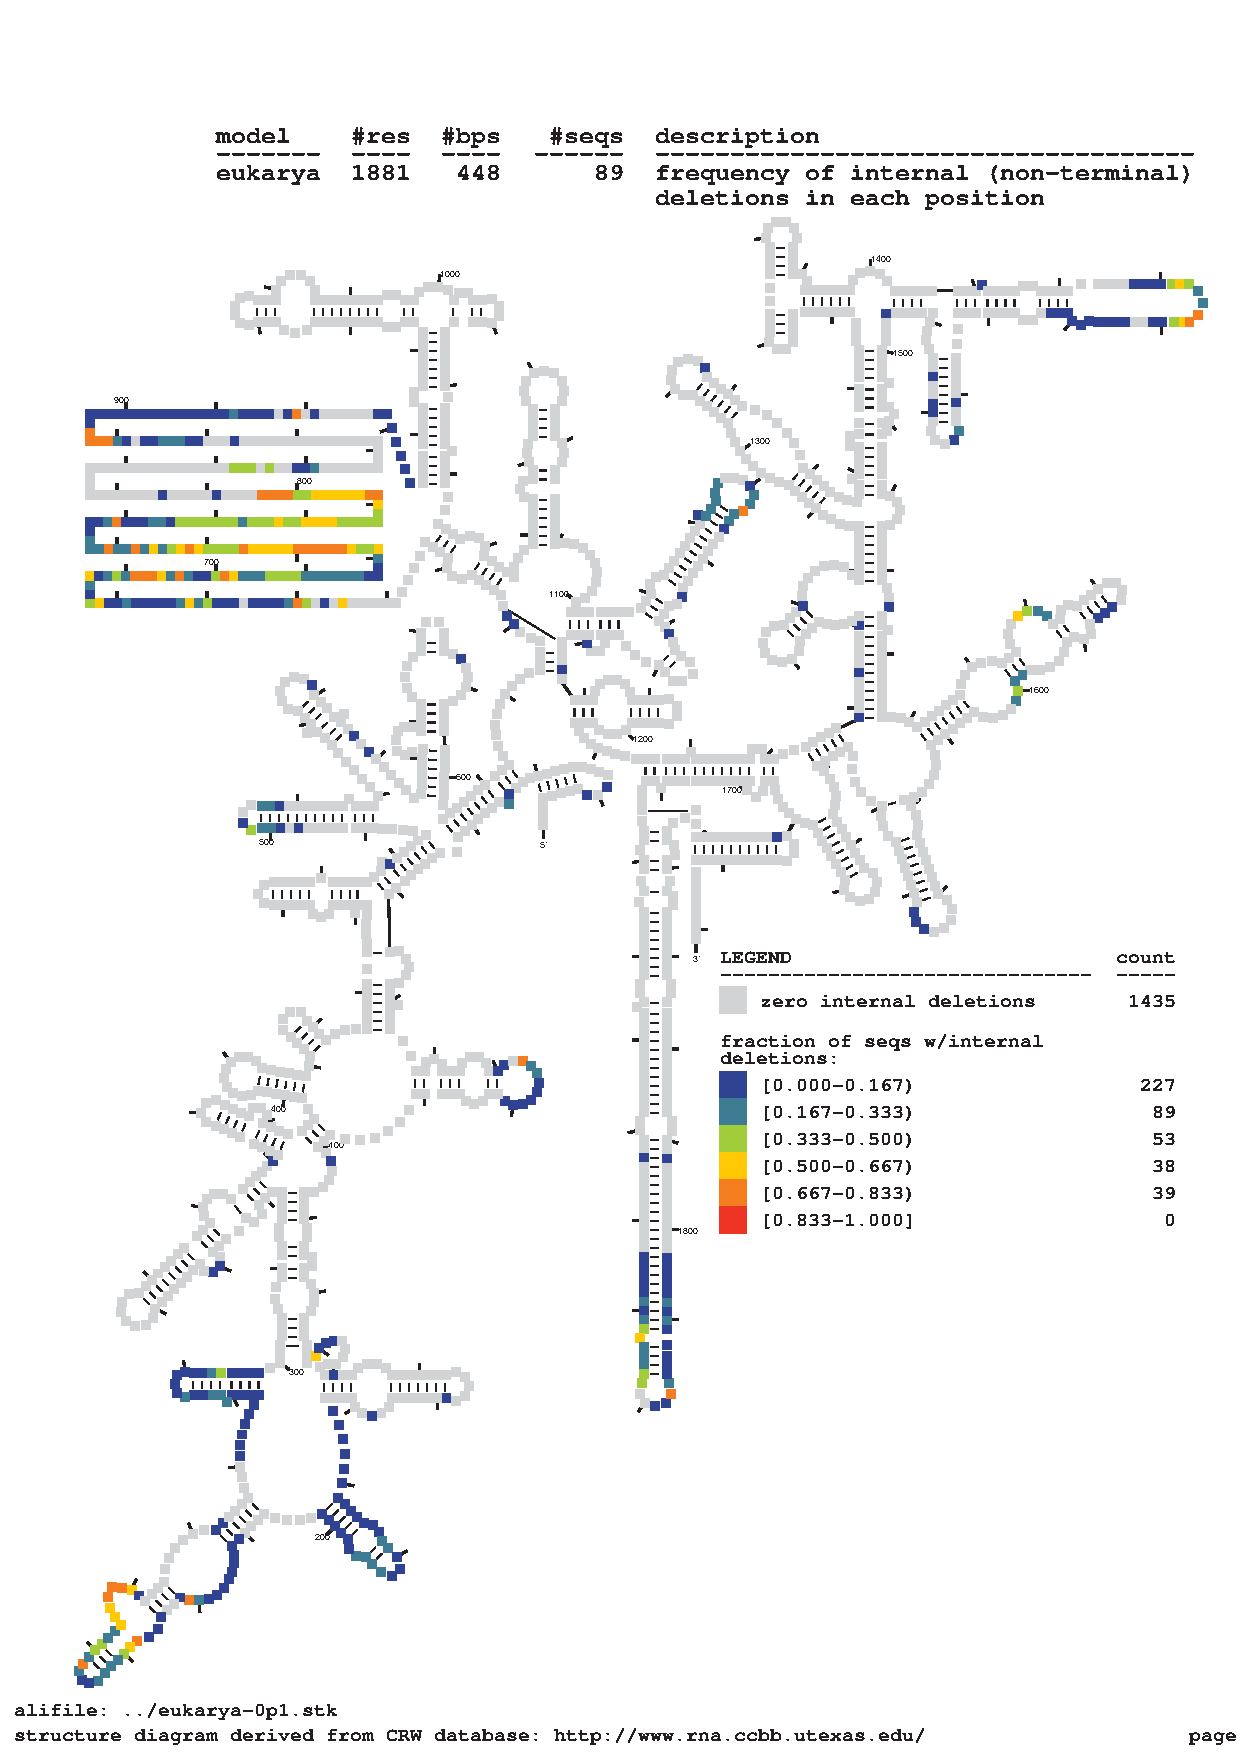
\includegraphics[height=8.5in]{Figures/eukarya-0p1-dint}
\label{fig:eukinfo}
\end{figure}

\newpage

\begin{figure}
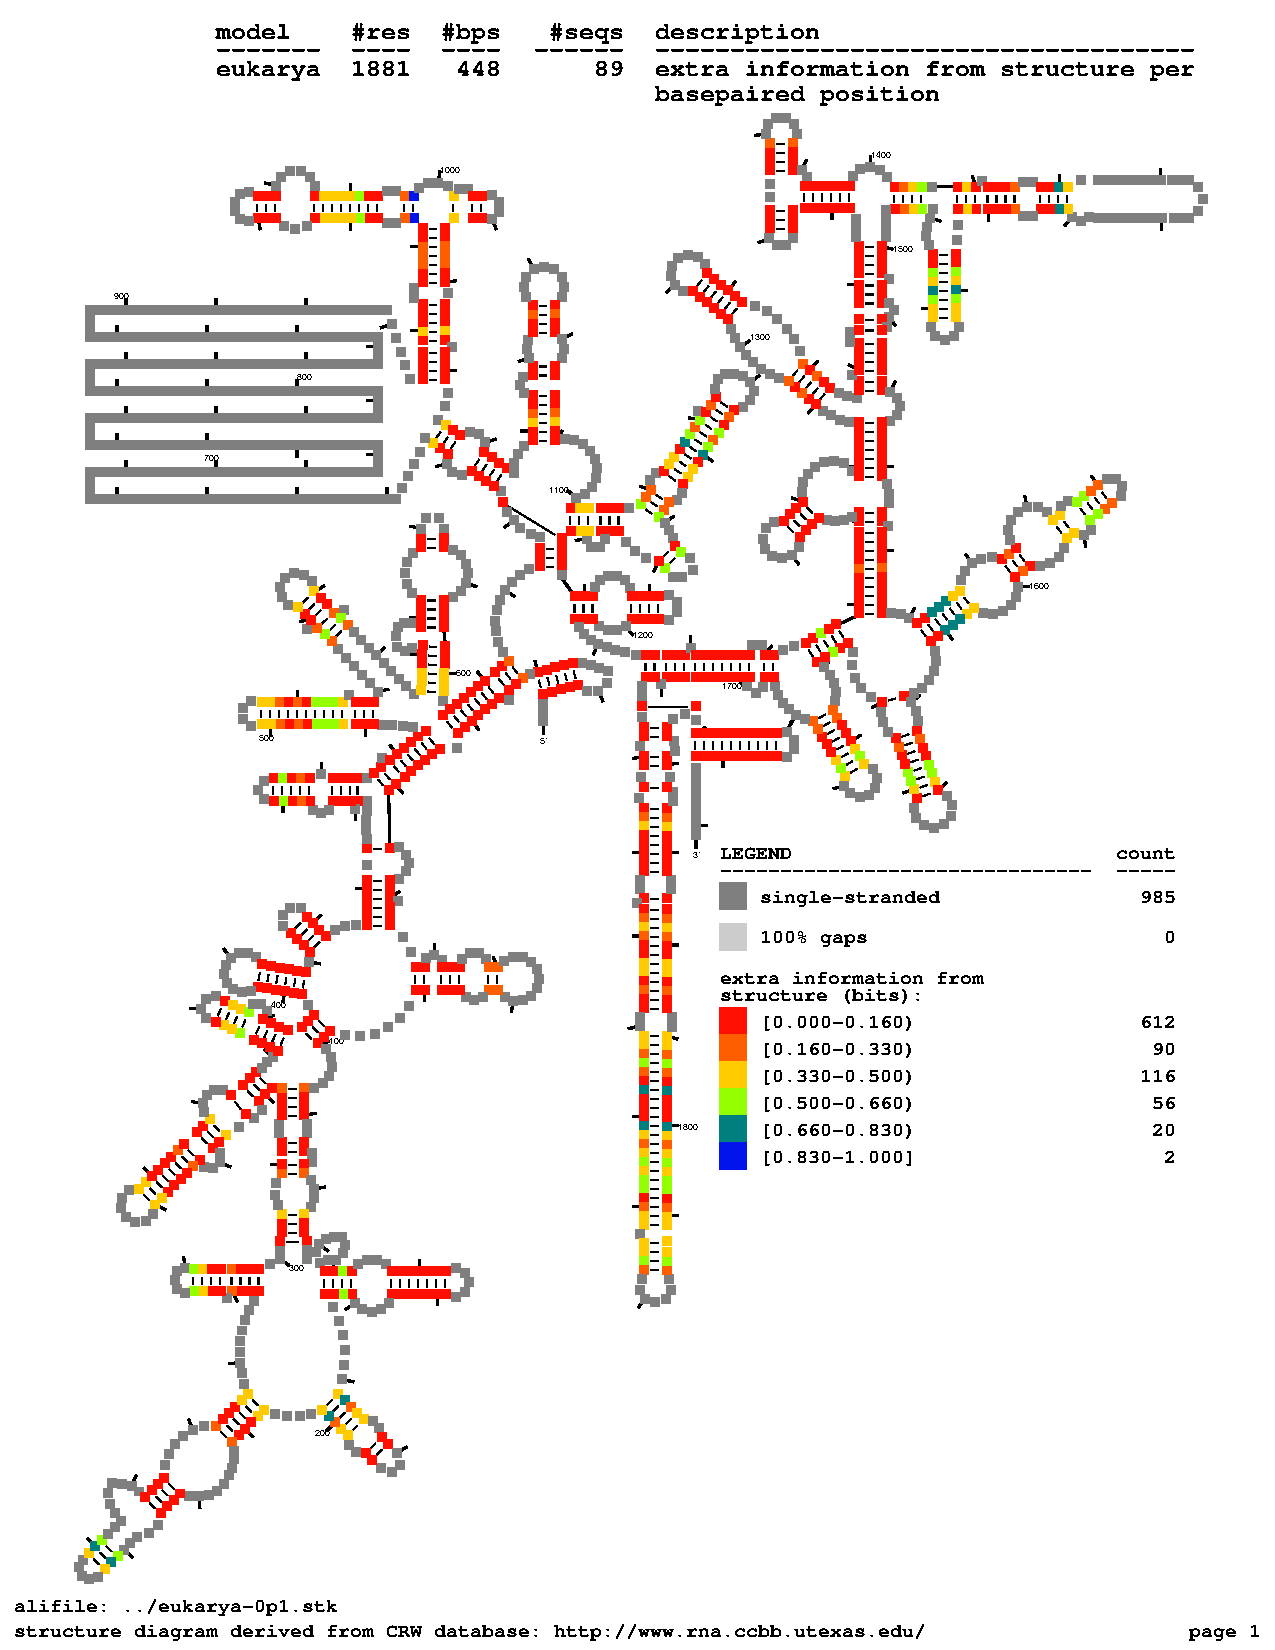
\includegraphics[height=8.5in]{Figures/eukarya-0p1-struct}
\label{fig:eukinfo}
\end{figure}









\subsection{Creating a truncated model of a specific region of SSU rRNA}

Many SSU rRNA sequencing studies target a specific region of the SSU
rRNA molecule using PCR primers at the boundaries of that region. For
such studies it is recommended to build a new CM that only models the
region of the molecule targetted by the study. There are two reasons
for this. The first is speed; the running time of \textsc{ssu-align}
decreases as the model size it's using decreases. The second reason is
that aligning a SSU subsequence to a model of only the region that
subsequence is derived from, relative to a model of the entire SSU
molecule, should slightly increase alignment accuracy. This is because
the uncertainty of what region of the full molecule the subsequence
should align to is eliminated. In this section I'll demonstrate how to
create a CM of a specific region of SSU and use it to create
alignments. 

For this example imagine our study is only targetting bacterial SSU
rRNA. We will use the bacterial SSU seed alignment that is included
with \textsc{ssu-align} as a starting point for creating our new,
truncated CM. The first step is to determine what consensus positions
in the bacterial seed alignment's consensus structure the targetted
region corresponds to. The consensus structure of the bacterial seed
alignment is shown in the ``Models'' section on page X.

Create a new directory and copy the bacterial seed alignment in
\prog{seeds/bacteria-0p1.stk}, the default parameters
file \prog{sa-0p1.params}, and the file \prog{tutorial/partial.fa}
there.

Let's say our 5' primer begins at consensus position 35 and our 3'
primer ends at position 397.  In practice, you'll have to manually
find your primer site and determine their positions on this consensus
structure. On the structure diagrams in the ``Models'' section, every
hundredth residue is numbered, and every tenth residue is marked with
a tick mark, which should help you find the relevant positions.  If
you have a subsequence that exactly spans from one primer to another,
you can align it to the appropriate \textsc{ssu-align} model, then
number the consensus positions of that alignment with
\prog{esl-alimanip --num-rf} and examine the numbered alignment to
determine the primer positions.

\begin{srefaq}{If I'm creating a truncated model for sequences derived
    using specific primers, should I include the primer sequences
    within the new model or not?} You should include the primers
  because they will help the program correctly align each
  sequence. The primer sites are very highly conserved so they are
  simple for the program to correctly align and anchor the alignment
  of the rest of the sequence.
\end{srefaq}

For this example, the first step towards creating a truncated model is
to create a truncated seed alignment that only models between
consensus positions 35 and 397. We can do this with the
\prog{esl-alimanip} program using the full bacterial seed alignment as
input:

\user{esl-alimanip --start-rf 35 --end-rf 397 -o bac-35-397.stk bacteria-0p1.stk}

This command creates a new alignment called \prog{back-35-397.stk} which
includes the subset of the columns from \prog{bacteria-0p1.stk} that lie
between consensus positions 35 and 397 inclusively.

The next step is to build a new model from this new alignment with
\textsc{infernal} 1.0's \prog{cmbuild} program. If this program is in
your path, you can execute it with \prog{cmbuild}, otherwise you'll
need to provide the full path. We will specify the name we want
to give the model with the \prog{-n} flag:

\user{cmbuild -n bac-35-397 --enone --gapthresh 0.8 bac-35-397.cm bac-35-397.stk}

\begin{srefaq}{Why did you specify \prog{--enone} and
    \prog{--gapthresh 0.8} as command-line flags to \prog{cmbuild}?}
    These are the recommended ``best-practice'' options for building
    models for SSU alignment. The \prog{--enone} flag tells the
    program to turn off entropy-weighting, a parameterization
    technique used to make CM homology search more sensitive
    \cite{Nawrocki07} but that seems slightly detrimental to CM
    alignment accuracy with SSU rRNA models. The \prog{--gapthresh
      0.8} flag tells the program to define any column that has less
    than 80\% gaps in the seed as a consensus column. Different values
    than 0.8 could be used here, but 0.8 empirically seems to yield
    good performance for SSU alignment. The \prog{--enone} and
    \prog{--gapthresh 0.8} flags were used to build
    \textsc{ssu-align}'s five default models in the \prog{seeds/}
    subdirectory of the package.
\end{srefaq}

Now you can begin using your new model \prog{bac-35-397.cm} to align
SSU sequences. You have two options.  You can either use your new
model by itself as the only model in an \prog{ssu-align} run, or you
can combine it with other models to create a multi-model file to use
with \prog{ssu-align}. The former option is recommended if you expect
all of your sequences to match the truncated model, e.g. in this case,
be bacterial SSU subsequences that map close to the 35-397
region. I'll run through an example of this below. The latter option,
combining this model with others, is recommended if only a subset of
the sequences you will analyze are expected to match the truncated
model. In that case, the other models you combine the truncated model
should span the diversity of the other sequences you expect in your
sequence dataset. (An example of using a multi-model file with
\textsc{ssu-align} is demonstrated in the basic tutorial section).

Imagine we expect all the sequences in our sequence dataset are
bacterial sequences that match near the 35-397 region. An example
sequence file with 8 such sequences derived from larger sequences in
the \prog{rocks.fa} file used in the basic tutorial is included in
\prog{partial.fa}. I artificially added 10 random residues to the 5\' and 3\'
ends of the 8th sequence to demonstrate that the program can 
trim residues it deems nonhomologous to the model from the ends of
the sequences before alignment.

\user{ssu-align bac-35-397.cm partial.fa single sa-0p1.params}

The program takes about 2 seconds to run. 

Take a look at the \prog{single.scores} file in the \prog{single/}
subdirectory:

\begin{sreoutput}
#                                                      best-matching model                 
#                                       -------------------------------------------------  
#     idx  sequence name                model name   beg   end    CM sc   struct   HMM sc
# -------  ---------------------------  ----------  ----  ----  -------  -------  -------
        1  gi|146141790|gb|EF522294.1|  bac-35-397     1   344   403.20   100.11   312.76
        2  gi|146141797|gb|EF522301.1|  bac-35-397     1   348   463.37    69.69   402.70
        3  gi|146141805|gb|EF522309.1|  bac-35-397     1   315   475.02    63.31   416.05
        4  gi|146141812|gb|EF522316.1|  bac-35-397     1   339   480.57    68.35   423.81
        5  gi|146141828|gb|EF522332.1|  bac-35-397     1   336   450.46    70.82   392.66
        6  gi|146141831|gb|EF522335.1|  bac-35-397     1   332   380.82    94.56   297.11
        7  gi|146141832|gb|EF522336.1|  bac-35-397     1   334   476.07    69.57   415.65
        8  gi|146141837|gb|EF522341.1|  bac-35-397    11   363   338.11    83.56   285.87
\end{sreoutput}

Note how the alignment of the final sequence begins at position 11 and
ends at 363, truncated the first and last 10 nonhomologous residues
that I had manually added (that sequence is 373 residues in
\prog{partial.fa}).


\subsection{Faster alignment of large datasets through parallelization
  with ssu-prep}
\label{sec:tutorial-prep}
\prog{ssu-align} runs on a single processor and does not support MPI
or multi-threading. However, if you have access to a compute
cluster or multi-core computers, simplistic parallelization is possible
with the \prog{ssu-prep} program.

\prog{ssu-prep} will split up a large input sequence file into
\emph{n} smaller files and create a shell script that will execute
\emph{n} \prog{ssu-align} jobs in parallel, each processing one of the
small sequence files. The results of all jobs will automatically be
merged together by the final job, ultimately yielding the same results
as if a single 
\prog{ssu-align}
job was run for the original large input sequence file. 
Parallelizing \prog{ssu-align} in this way can drastically reduce the
actual time required for aligning large datasets. A job that would
have required 100 hours on 1 processor can be done in a little more
than 1 hour on 100 processors. See table~\ref{tbl:ttimes} in
section~\ref{sec:stats} for example timing statistics. 

In this section we'll walk through an example of how to do this for a
small dataset.  The sequence file \prog{tutorial/seed-30.fa} includes
30 randomly chosen sequences from the complete set of seed sequences
from the three default models of \textsc{ssu-align}.

\prog{ssu-prep} has three different usage modes as explained by the
program if it is run without any command-line arguments:

\user{ssu-prep}

\begin{sreoutput}
Incorrect number of command line arguments.
Usage: ssu-prep    [-options] <seqfile> <output dir> <num jobs> <prefix/suffix file>
Usage: ssu-prep -x [-options] <seqfile> <output dir> <num jobs>
Usage: ssu-prep -y [-options] <seqfile> <output dir> <num jobs>

ssu-prep splits up <seqfile> into <num jobs> smaller files and creates a shell
script that will execute <num jobs> ssu-align jobs in parallel, each processing
one of the small sequence files. The results of all jobs will automatically be
merged together by the final job, giving the same results as if a single
ssu-align job was run for the complete <seqfile>.

The 3 different usages control how the prefix and suffix are defined for the jobs
in the output shell script, allowing, for example, the user to wrap the ssu-align
commands in a cluster submission command (such as Sun Grid Engine's "qsub"):

Default: (neither -x nor -y enabled) prefix and suffix for ssu-align jobs in
         output shell script are defined in <prefix/suffix file>. First line is
         the prefix, second line is the suffix.
With -x: do not specify <prefix/suffix file>; output shell script will run all
         <num jobs> jobs in parallel on one machine with <num jobs> cores/cpus.
With -y: do not specify <prefix/suffix file>; user will manually add the desired
         prefix/suffix to ssu-align commands after ssu-prep finishes.

To see more help on available options, do ssu-prep -h
\end{sreoutput}

By default, if neither \prog{-x} nor \prog{-y} options are used, the program
reads a \prog{<prefix/suffix file>}, a simple two line file that
a prefix string and a suffix string to prepend and append respectively
to the \prog{ssu-align} commands it generates. 

The strings in the \prog{<prefix/suffix file>} will likely be specific
to your parallel computing environment. At Janelia, we use Sun Grid
Engine's \prog{qsub} program for submitting jobs to a large compute
cluster. The relevant prefix/suffix file for our specific
computing environment is included in \\
\prog{tutorial/janelia-cluster-presuf.txt}. Take a look at this file:

\begin{sreoutput}
qsub -N ssu-align -o /dev/null -b y -j y -cwd -V "
"
\end{sreoutput}

The first line is the prefix string, containing the name and
appropriate command line arguments of the \prog{qsub} program which
submits jobs to the Grid Engine queuing system at Janelia. The second
line is the suffix, and contains only a double quote, which
complements the double quote at the end of the prefix line as we'll
see below.

Now, let's run \prog{ssu-prep} as if we were going to create parallel
\prog{ssu-align} jobs for the Janelia cluster.  Move into the
\prog{tutorial/} directory and execute the command:

\user{ssu-prep seed-30.fa my30 5 janelia-cluster-presuf.txt}

About forty lines of text are output to the screen. We'll step through
and discuss this output: 

\begin{sreoutput}
# Validating input sequence file ... done.
#
# Preparing 5 ssu-align jobs ...
# Partitioning seqs with goal of equalizing total number of nucleotides per job ...
#
# output file name   description                                       
# -----------------  --------------------------------------------------
  my30/seed-30.fa.1  partition 1 FASTA sequence file (6 seqs; 10463 nt)
  my30/seed-30.fa.2  partition 2 FASTA sequence file (6 seqs; 10240 nt)
  my30/seed-30.fa.3  partition 3 FASTA sequence file (6 seqs;  9922 nt)
  my30/seed-30.fa.4  partition 4 FASTA sequence file (6 seqs; 10358 nt)
  my30/seed-30.fa.5  partition 5 FASTA sequence file (6 seqs;  9397 nt)
  my30.ssu-align.sh  shell script that will execute 5 ssu-align jobs
#
\end{sreoutput}

First, \prog{ssu-prep} reports that it has validated the formatting of
the sequence file, partitioned it into 5 new files and placed each file
into the newly created \prog{my30/} subdirectory. Each of these files has
6 of the original 30 sequences in it. Additionally,
\prog{my30.ssu-align.sh}, a shell script that will execute 5 jobs, one
per sequence file, was created in the current working directory. After
this, you'll see:

\begin{sreoutput}
################################################################################
# To execute all 5 ssu-align jobs, run the shell script with:
#	sh my30.ssu-align.sh
################################################################################
\end{sreoutput}

These are instructions for how to execute the shell script. Take a
look at the shell script \\ \prog{my30.ssu-align.sh}:

\begin{sreoutput}
#!/bin/bash
# Bash shell script created by ssu-prep for running 5 ssu-align jobs.
# Each job will process a separate partition of the sequence file:
# 'seed-30.fa'.
#
# The final job is special, after computing its alignments it will wait for all
# other jobs to finish and then merge the output of all jobs together.
# The merged output files will be in the directory: '/my30/'
#
# The for loop below will execute/submit the first 4 of 5 jobs.
# The final ssu-align job is executed separately because it does the merging.
#
for i in {1..4}
do
	echo "# Executing: qsub -N ssu-align -o /dev/null -b y -j y -cwd -V " ssu-align my30/seed-30.fa.$i my30/my30.$i ""
	qsub -N ssu-align -o /dev/null -b y -j y -cwd -V " ssu-align my30/seed-30.fa.$i my30/my30.$i "
done
echo "# Executing: qsub -N ssu-align -o /dev/null -b y -j y -cwd -V " ssu-align --merge 5 my30/seed-30.fa.5 my30/my30.5 ""
qsub -N ssu-align -o /dev/null -b y -j y -cwd -V " ssu-align --merge 5 my30/seed-30.fa.5 my30/my30.5 "
\end{sreoutput}

This is a bash shell script file\footnote{The \prog{--no-bash} option
  can be used to make a non-bash-specific script, see the
  \prog{ssu-prep} manual page for more information.}.
The \prog{\#}-prefixed lines are
explanatory comments. The remainder of the file consists of a for loop
that will submit the first four \prog{ssu-align} jobs to the cluster
using \prog{qsub}. The lines beginning with \prog{qsub} are the actual
job submission commands. The lines beginning with \prog{echo} cause updates to
be printed to STDOUT before each job is submitted. 
Note that the \prog{qsub} command line is composed
of the prefix string from the \prog{janelia-cluster-presuf.txt} file,
followed by a \prog{ssu-align} command, followed by the suffix
string. The end result is that the \prog{ssu-align} command is
contained within the quotes from the prefix/suffix strings.

The comments explain that the final job is special. It will merge the
results of all jobs once they are finished. Consequently, it requires
special command-line options and so is executed outside the for loop,
as the final line of the script.

%%%%%%%%%%%%%%%%%%%%%%%%%%%%%%%%%%%%%%%%%%%%%%%%%%%%%%%%%%%%%%%%%%%%%
\begin{comment}
The final important part of the \prog{ssu-prep} output explains what
to do if any of the jobs fail: 

\begin{sreoutput}
# If one or more jobs fail: rerun the failed jobs, wait for them to finish,
# and then perform manual merge from this directory by executing:
#	ssu-merge my30
\end{sreoutput}

This should happen only rarely, but if any jobs fail, this aspect of
the program allows 
\end{comment}
%%%%%%%%%%%%%%%%%%%%%%%%%%%%%%%%%%%%%%%%%%%%%%%%%%%%%%%%%%%%%%%%%%%%%

Because your specific compute system is likely different from
Janelia's, the \prog{my30.ssu-align.sh} script will probably not
work. To make \prog{ssu-prep} generate shell scripts you can run on
your system, create a file like \prog{janelia-cluster-presuf.txt} but
with prefix and suffix strings specific to your
system. 

This simple prefix/suffix string method may not work for your
compute system. For example, if your cluster requires using \prog{ssh}
to remote login to different nodes, a single fixed prefix line will
probably not be sufficient. If this is the case, run \prog{ssu-prep}
with the \prog{-y} option. In this mode no prefix/suffix file
will be read, and the output shell script will contain only the raw
\prog{ssu-align} commands. For example, do:

\user{ssu-prep -f -y seed-30.fa my30 5}

(We had to also specify \prog{-f} so the program would overwrite our
existing \prog{my30} directory.) Much of the output is the same as the
prior example, but the \prog{WARNING} section is new:

\begin{sreoutput}
################################################################################
# WARNING: -y was set on the command line.
# This means that 'my30.ssu-align.sh' will simply run the 5 ssu-align jobs in
# succession, one after another, not in parallel. If you want to run the jobs in
# parallel you'll either have to manually edit that file or rerun ssu-prep using
# the options listed above to specify prefix and/or suffix strings for the
# ssu-align commands, so they are, for example, submitted to run on a cluster
# using a queing system manager like SGE. Or you can run <n> jobs in parallel on
# a single <n>-core machine by rerunning ssu-prep using '-x'.
# Do 'ssu-prep -h' or see the User Guide for more information.
################################################################################
\end{sreoutput}

As explained, you'll have to modify the newly created
\prog{my30.ssu-align.sh} to make the jobs run in parallel in this
case, either manually or using your own script. The file will still
contain a for loop submitting all but the final job. If you'd rather
all jobs were placed on their own line, use the \prog{--no-bash}
option to \prog{ssu-prep}.

For now, let's run the unmodified \prog{my30.ssu-align.sh} script to
demonstrate how the jobs are merged together automatically. As noted
in the warning above, this will simply run the 5 jobs in succession
instead of in parallel, but for our purposes here this is okay. To run
the script, execute the command: 

\user{sh my30.ssu-align.sh \footnote{If this command fails, you're
    probably not using the BASH shell. Rerun the \prog{ssu-prep}
    command above with the \prog{--no-bash} option and try again.}}

The script executes \prog{ssu-align} five times in succession, and
these jobs will being reporting what they're doing to the screen. 
Once all five jobs are run, the \prog{ssu-merge} program will
automatically be called to merge their output. You'll see the
following output at that point:

\begin{sreoutput}
# Merging files from 5 ssu-align runs...
#
#                                  # files     # seqs
# merged file name       CM name    merged     merged
# ---------------------  --------  -------  ---------
  my30.tab               -               5          -
  my30.scores            -               5          -
  my30.ssu-align.sum     -               5          -
  my30.ssu-align.log     -               5          -
#
  my30.archaea.fa        archaea         2          5
  my30.archaea.hitlist   archaea         2          5
  my30.archaea.cmalign   archaea         2          5
  my30.archaea.ifile     archaea         2          5
  my30.archaea.stk       archaea         2          5
#
  my30.bacteria.fa       bacteria        5          8
  my30.bacteria.hitlist  bacteria        5          8
  my30.bacteria.cmalign  bacteria        5          8
  my30.bacteria.ifile    bacteria        5          8
  my30.bacteria.stk      bacteria        5          8
#
  my30.eukarya.fa        eukarya         5         17
  my30.eukarya.hitlist   eukarya         5         17
  my30.eukarya.cmalign   eukarya         5         17
  my30.eukarya.ifile     eukarya         5         17
  my30.eukarya.stk       eukarya         5         17
\end{sreoutput}

Two of the five small partition files included archaeal sequences, and
all five included bacterial and eukaryotic  sequences. The total number
of archaeal, bacterial and eukaryotic sequences was 5, 8 and 17,
respectively. The final merged alignments are in the files
\prog{my30.archaea.stk}, \prog{my30.bacteria.stk}, and
\prog{my30.eukarya.stk}.

subsubsection{Using ssu-prep to parallelize ssu-align
  on multi-core machines}

The third and final \prog{ssu-prep} usage mode is for parallelizing
jobs to run on a single multi-core machine. This mode can be thought
of as a simple substitute for multi-threading, and is enabled with the
\prog{-x} option to \prog{ssu-prep}. As with \prog{-y}, using
\prog{-x} obviates the need for a prefix/suffix file. As an example,
imagine you are using a quad-core machine. In this case, execute: 

\user{ssu-prep -f -x seed-30.fa my30 4}

(We had to also specify \prog{-f} so the program would overwrite our
existing \prog{my30} directory.) Much of the output is the same as
before. However, the \prog{my30.ssu-align.sh} file will be different;
it is included below:

\begin{sreoutput}
#!/bin/bash
# Bash shell script created by ssu-prep for running 4 ssu-align jobs.
# Each job will process a separate partition of the sequence file:
# 'seed-30.fa'.
#
# This script will execute all 4 jobs at once, in parallel. It is only
# meant to be executed on a system with 4 cpus/cores. The first 3 jobs
# will run in the background and output to /dev/null. The final job will
# output to STDOUT, allowing you to follow its progress.
#
# The final job is special, after computing its alignments it will wait for all
# other jobs to finish and then merge the output of all jobs together.
# The merged output files will be in the directory: '/my30/'
#
# The for loop below will execute/submit the first 3 of 4 jobs.
# The final ssu-align job is executed separately because it does the merging.
#
for i in {1..3}
do
	echo "# Executing: ssu-align my30/seed-30.fa.$i my30/my30.$i > /dev/null &"
	ssu-align my30/seed-30.fa.$i my30/my30.$i > /dev/null &
done
echo "# Executing: ssu-align --merge 4 my30/seed-30.fa.4 my30/my30.4"
ssu-align --merge 4 my30/seed-30.fa.4 my30/my30.4
\end{sreoutput}

Note that the \prog{ssu-align} commands in the for loop include
\prog{\&} at the end, which cause them to be run simultaneously.











\subsection{Merging multiple alignments together}

INFERNAL's \prog{cmalign} program is capable of merging
two alignments into one. The two alignments must have both been
created by \prog{cmalign} (and the same version of \prog{cmalign}, 1.0
or later), and must have been created using the same exact CM. This
ability is potentially useful for saving time when aligning a large
number of sequences if you have access to a compute cluster, as
described in the previous section (``Splitting up large alignment
jobs''), or if you want to merge an existing reference alignment with
a newly created one, which is demonstrated below. Combining a new
alignment with a reference one may be useful in downstream
phylogenetic analysis, for example, if you know the classification of
the sequences in the reference alignment.

Imagine we wanted to merge the bacterial sequences from the 
\prog{seed-15} alignment we created at the beginning of the tutorial
with a single sequence alignment of the commonly used reference
sequence \emph{E. coli} \db{genbank} accession J01695. 

Merging alignments only makes sense and saves time if you've already
computed at least one of the two alignments you want to merge. For
this example I've provided the two alignments in the \\
\prog{infernal-1.01/ssu-align-0.1/tutorial} directory:

\begin{description}
\item[\emprog{seed-15.bacteria.stk}]
  An alignment of the five bacterial sequences from the \prog{seed-15.fa}
  sequence file. The beginning of this tutorial steps through how to create this file.

\item[\emprog{ecoli.bacteria.stk}]
  An alignment of the single J01695 bacterial sequence. This was
  created by aligning the sequence with the default bacterial CM.
\end{description}

To merge these two alignments into a single alignment called
\prog{seed-15-ecoli.bacteria.stk}, create or move
into the directory \prog{infernal-1.01/ssu-align-0.1/my-tutorial}, and
execute: 

\user{../../src/cmalign --merge -o seed-15-coli.bacteria.stk \\
../seeds/bacteria-0p1.cm ../tutorial/seed-15.bacteria.stk \\ ../tutorial/ecoli.bacteria.stk}

The resulting alignment will be 100\% identical to the alignment
\prog{cmalign} would have created if it were used to align a single
sequence file that included the five seed-15 sequences and the J01695
sequence together.









